\documentclass{book}

\usepackage{ctex}
\usepackage{amsmath}
\usepackage{physics}
\usepackage{listings}
\usepackage{graphicx}
\usepackage[dvipsnames]{xcolor}
\usepackage{chemformula}
\usepackage{amsthm}
\usepackage{siunitx}

\title{数值分析笔记\\Python version}
\author{Jiaqi Z.}

\newtheorem{theorem}{\indent 定理}[section]
\newtheorem{lemma}[theorem]{\indent 引理}
\newtheorem{proposition}[theorem]{\indent 命题}
\newtheorem{corollary}[theorem]{\indent 推论}
\newtheorem{definition}{\indent 定义}[section]
\newtheorem{example}{\indent 例}[section]
\newtheorem{remark}{\indent 注}[section]
\newenvironment{solution}{\begin{proof}[\indent\bf 解]}{\end{proof}}
\newenvironment{notice}{\textbf{注意: }}{}
\newenvironment{extend}{\itshape 扩展: }{}
\renewcommand{\proofname}{\indent\bf 证明}

\newcommand{\approxstar}[1]{#1^*}

% 代码环境设置

\lstset{
    language=Python, % 设置语言
 basicstyle=\ttfamily, % 设置字体族
 breaklines=true, % 自动换行
 keywordstyle=\bfseries\color{NavyBlue}, % 设置关键字为粗体,颜色为 NavyBlue
 morekeywords={}, % 设置更多的关键字,用逗号分隔
 emph={self}, % 指定强调词,如果有多个,用逗号隔开
    emphstyle=\bfseries\color{Rhodamine}, % 强调词样式设置
    commentstyle=\itshape\color{black!50!white}, % 设置注释样式,斜体,浅灰色
    stringstyle=\bfseries\color{PineGreen!90!black}, % 设置字符串样式
    columns=flexible,
    numbers=left, % 显示行号在左边
    numbersep=2em, % 设置行号的具体位置
    numberstyle=\footnotesize, % 缩小行号
    frame=single, % 边框
    framesep=1em % 设置代码与边框的距离
}

\begin{document}
    \maketitle
    \tableofcontents
    \chapter{绪论}
\section{误差}

\subsection{误差来源与分类}
\begin{enumerate}
    \item (\emph{模型误差}):从实际模型中抽象出数学模型;
    
    例如, 一个质量为$m$的小球做自由落体运动, 则位置$s$与时间$t$的关系式满足:
    \begin{equation*}
        m\dv[2]{s}{t}=mg
    \end{equation*}
    不难想见, 该式仅在\emph{不考虑阻力}时成立.

    \item (\emph{观测误差}):通过测量得到模型中参数的值;
    \item (\emph{方法误差}(或称\emph{截断误差})):求近似解时所引入的误差;
    \begin{example}
        考虑函数$f(x)$做Taylor多项式展开所导致的截断误差.
    \end{example}
    \begin{solution}
        对函数$f(x)$计算Taylor多项式, 有
        \begin{equation*}
            P_n(x)=f(0)+\frac{f'(0)}{1!}x+\frac{f''(0)}{2!}x^2+\cdots+\frac{f^{(n)}(0)}{n!}x^n
        \end{equation*}
        由于有限项, 因此多项式有截断误差
        \begin{equation*}
            R_n(x)=\frac{f^{(n+1)}(\xi)}{(n+1)!}x^{n+1}
        \end{equation*}
        其中, $\xi\in(x,0)$
    \end{solution}

    \item (\emph{舍入误差}):机器字长有限所引起的误差 
\end{enumerate}

其中, \emph{方法误差}和\emph{舍入误差}是数值分析所重点考虑的误差, 同时, \emph{方法误差是可以避免的}.

\subsection{误差概念}
\subsubsection{绝对误差与绝对误差限}
\begin{definition}[绝对误差与绝对误差限]
    设$x$是准确值, $x^*$是$x$的一个近似值, 则称
    \begin{equation*}
        e(x^*)=x^*-x
    \end{equation*}
    为$x^*$的\emph{绝对误差}, 简称\emph{误差}.

    同时, 误差的绝对值的上限$\varepsilon(x^*)$, 即有
    \begin{equation*}
        \abs{e(x^*)}=\abs{x^*-x}\le\varepsilon(x^*)
    \end{equation*}

    $\varepsilon(x^*)$称为\emph{绝对误差限}.
\end{definition}

\begin{notice}
    误差有正有负, 而误差限恒为正值.
\end{notice}

习惯上, 我们把精确值和测量值的关系表示为
\begin{equation*}
    x=x^*\pm\varepsilon
\end{equation*}

\subsubsection{相对误差与相对误差限}

\begin{definition}[相对误差与相对误差限]
    设$x$为准确值, $x^*$为近似值, 称
    \begin{equation*}
        e_r^*=e_r^*(x^*)=\frac{e(x^*)}{x}=\frac{x^*-x}{x}
    \end{equation*}
    为近似值$x^*$的\emph{相对误差}.

    同时, 其绝对值的上限$\varepsilon_r^*$, 即有
    \begin{equation*}
        \abs{\frac{x-x^*}{x}}\le \varepsilon_r^*
    \end{equation*}
    
    $\varepsilon_r^*$称为\emph{相对误差限}.
\end{definition}

可以证明, 当$e_r^*$较小时, 有
\begin{equation*}
    e_r^* \approx\frac{x^*-x}{x^*}
\end{equation*}
同时易得
\begin{equation*}
    \varepsilon_r^*=\frac{\varepsilon^*}{\abs{x^*}}
\end{equation*}

\subsubsection{有效数字}

\begin{definition}[有效数字, 有效位数, 有效数]
    若近似值$x^*$误差满足
    \begin{equation*}
        \abs{x-x^*}\le\frac{1}{2}\times10^{-n}
    \end{equation*}
    则称$x^*$近似表示$x$准确到小数点后第$n$位, 并从第$n$位起一直到最左边非零数字之间的一切数字称为\emph{有效数字}, 位数为\emph{有效位数}.

    若所有数字均为有效数字, 则称为\emph{有效数}
\end{definition}

\begin{example}
    考虑圆周率$\pi$, 且有近似值$\pi_1=3.14, \pi_2=3.1415, \pi_3=3.1416, \pi_4=3.14159$. 考虑它们的有效数字, 且判断是否为有效数.
\end{example}

\begin{solution}
    对于$\pi_1=3.14$, 有$\abs{\pi-\pi_1}\approx0.00159\le0.5\times10^{-2}$, 即$\pi_1$精确到小数点后2位, 有效数字是3位, 是有效数.

    同理, 有$\abs{\pi-\pi_2}\approx0.0000926\le0.5\times10^{-3}$, 即$\pi_2$精确到小数点后3位, 有效数字是4位, 不是有效数.

    $\abs{\pi-\pi_3}\approx0.0000073\le0.5\times10^{-4}$, 即$\pi_3$精确到小数点后4位, 有效数字是5位, 是有效数.

    $\abs{\pi-\pi_4}\approx0.0000026\le0.5\times10^{-5}$, 即$\pi_4$精确到小数点后5位, 有效数字是6位, 是有效数.
\end{solution}

从上例中不难看出, 有效数通常是采取\emph{四舍五入}所得到的近似值.

\begin{extend}
    我们可以简单给出关于\emph{四舍五入}的证明.

    \begin{proof}
        设准确值为$x$, 其近似值为$x^*$, 考虑近似值精确到小数点后$n$位, 即
        \begin{equation*}
            \abs{x-x^*}\le5\times10^{-(n+1)}
        \end{equation*}

        若其为有效数, 则$x^*$为小数点后$n$位, 不妨设
        \begin{equation*}
            x^*=a+b\cdot10^{-n}
        \end{equation*}
        其中$b\in[1,10)$

        特别地, 分两种情况讨论. 

        若$x>x^*$, 即真实值大于近似值, 此时有
        \begin{equation*}
            x\le x^*+5\times10^{-(n+1)}=a+b\cdot10^{-n}+5\times10^{-(n+1)}
        \end{equation*}
        即当小数点后第$n+1$位小于等于5时, 舍去后面的数字可以得到有效数.

        若$x<x^*$, 即真实值小于近似值, 此时有
        \begin{align*}
            x\ge x^*-5\times10^{-(n+1)}&=a+b\cdot10^{-n}-5\times10^{-(n+1)}\\
            &=a+(b-1)\cdot10^{-n}+5\times10^{-(n+1)}
        \end{align*}
        即当小数点后第$n+1$位大于等于5时, 进位可以得到有效数.
    \end{proof}
\end{extend}

\subsubsection{十进制浮点表示法}

\begin{definition}
    设$x^*$为任一十进制数, 则$x^*$可表示为
    \begin{equation*}\label{eqn:1.3.1}
        x^*=\pm0.a_1a_2\cdots a_n\cdots\times10^m
    \end{equation*}
    其中, $a_1$为1到9之间的一个数字, $a_2\cdots a_n$为0到9之间的一个数字, $m$为整数. 这样表示的$x^*$称为\emph{十进制浮点数(规格化浮点数)}.
\end{definition}

\subsubsection{有效数字的等价定义(基于浮点表示法)}

\begin{definition}
    若近似值$x^*=\pm0.a_1a_2\cdots a_na_{n+1}\cdots a_{n+p}\times10^m(a_1\ne0)$的误差限是某一位上的半个单位, 即
    \begin{equation}\label{eqn:有效数字的等价定义}
        \abs{x-x^*}\le\frac{1}{2}\times10^{m-n}
    \end{equation}
    则称$x^*$有$n$位有效数字.
\end{definition}

\begin{example}
    设$x_1^*=0.0051, x_2^*=5.100$, 两数均为四舍五入得到, 求两个数字的有效位数.
\end{example}
\begin{solution}
    由于有
    \begin{align*}
        \varepsilon(x_1^*)&=0.5\times10^{-4}, x_1^*=0.51\times10^{-2}\\
        \varepsilon(x_2^*)&=0.5\times10^{-3}, x_2^*=0.51\times10^1
    \end{align*}
    可得
    \begin{align*}
        \varepsilon(x_1^*)&=0.5\times10^{-2-2}\\
        \varepsilon(x_2^*)&=0.5\times10^{1-4}
    \end{align*}
    即, $x_1^*$有两位有效数字, $x_2^*$有四位有效数字.
\end{solution}

\begin{example}
    设$x_1^*=2.180, x_2^*=10.210$, 均具有四位有效数字, 求绝对误差限和相对误差限.
\end{example}

\begin{solution}
    对$x_1^*$, 有
    \begin{equation*}
        x_1^*=0.2180\times10^1
    \end{equation*}
    即$m=1$, 且具有四位有效数字, 即$n=4$, 则根据公式(\ref{eqn:有效数字的等价定义}), 有
    \begin{equation*}
        \varepsilon(x_1^*)=0.5\times10^{1-4}=0.5\times10^{-3}
    \end{equation*}
    其相对误差限为
    \begin{equation*}
        \varepsilon_r(x_1^*)=\frac{\varepsilon(x_1^*)}{\abs{x_1^*}}=0.023\%
    \end{equation*}

    同理可得, 对于$x_2^*$, 有
    \begin{equation*}
        \varepsilon(x_2^*)=0.5\times10^{-2}, \varepsilon_r(x_2^*)=0.049\%
    \end{equation*}
\end{solution}

\subsection{相对误差限和有效数字的关系}

关于有效数字和相对误差限之间的关系, 有如下定理.
\begin{theorem}\label{dingli1.1}
    对于用式(\ref{eqn:1.3.1})表示的近似数$x^*$, 若$x^*$具有$n$位有效数字, 则其相对误差限为
    \begin{equation*}
        \varepsilon_r^*\le\frac{1}{2a_1}\times10^{-n}
    \end{equation*}
\end{theorem}

\begin{proof}
    由式\ref{eqn:1.3.1}可得
    \begin{equation*}
        a_1\times10^m\le\abs{x^*}\le(a_1+1)\times10^m
    \end{equation*}
    当$x^*$有$n$位有效数字时, 有
    \begin{equation*}
        \abs{x-x^*}=\abs{x^*}\varepsilon_r^*\le(a_1+1)\times10^m\times\frac{1}{2(a_1+1)}\times10^{-n}=0.5\times10^{m-n}
    \end{equation*}
    故$x^*$有$n$位有效数字.
\end{proof}

上述定理表明: \emph{有效位数越多, 相对误差限越小}.

\begin{example}
    令$\sqrt{20}$的近似值相对误差限小于0.1\%, 则需要取多少位有效数字?
\end{example}
\begin{solution}
    由定理\ref{dingli1.1}可知
    \begin{equation*}
        \varepsilon_r^*\le\frac{1}{2a_1}\times10^{-n}
    \end{equation*}
    由于$\sqrt{20}\approx4.4$, 故$a_1=4$, 只需要取$n=4$, 有
    \begin{equation*}
        \varepsilon_r^*\le0.125\times10^{-3}<10^{-3}=0.1\%
    \end{equation*}
    即只需要对$\sqrt{20}$的近似值取4位有效数字, 其相对误差限就可以小于0.1\%, 此时有
    \begin{equation*}
        \sqrt{20}\approx4.472.
    \end{equation*}
\end{solution}

\section{数值运算的误差估计}

\subsection{四则运算误差估计}

两个近似数分别为$x_1^*$和$x_2^*$, 误差限分别为$\varepsilon(x_1^*),\varepsilon(x_2^*)$, 进行四则运算的误差限分别为:
\begin{align*}
    \varepsilon(x_1^*\pm x_2^*)&=\varepsilon(x_1^*)+\varepsilon(x_2^*)\\
    \varepsilon(x_1^*x_2^*)&\approx\abs{x_1^*}\varepsilon(x_2^*)+\abs{x_2^*}\varepsilon(x_1^*)\\
    \varepsilon(x_1^*/x_2^*)&\approx\frac{\abs{x_1^*}\varepsilon(x_2^*)+\abs{x_2^*}\varepsilon(x_1^*)}{\abs{x_2^*}^2}
\end{align*}

下面试着给出加减法误差的证明, 对于乘法和除法的证明, 将在后面给出.

\begin{proof}
    \begin{align*}
        \abs{e(x_1^*\pm x_2^*)}&=\abs{(x_1^*\pm x_2^*)-(x_1\pm x_2)}\\
        &=\abs{(x_1^*-x_1)\pm(x_2^*-x_2)}\\
        &\le\abs{x_1^*-x_1}+\abs{x_2^*-x_2}\\
        &\le\varepsilon(x_1^*)+\varepsilon(x_2^*)
    \end{align*}
\end{proof}

\subsection{函数值误差估计}

\subsubsection{一元函数误差估计}

设$f(x)$是一元函数, $x$的近似值为$x^*$, 以$f(x^*)$近似$f(x)$, 其误差限记作$\varepsilon(f(x^*))$, 可用Taylor展开
\begin{equation*}
    f(x)-f(x^*)=f'(x^*)(x-x^*)+\frac{f''(\xi)}{2}\varepsilon^2(x^*)
\end{equation*}
其中, $\xi$介于$x, x^*$之间, 取绝对值有
\begin{equation*}
    \abs{f(x)-f(x^*)}\le\abs{f'(x^*)}\varepsilon(x^*)+\frac{\abs{f''(\xi)}}{2}\varepsilon^2(x^*)
\end{equation*}

假定$f'(x^*)$与$f''(x^*)$的比值不大, 可忽略$\varepsilon(x^*)$的高阶项, 于是可得误差限为
\begin{equation*}
    \varepsilon(f(x^*))\approx\abs{f'(x^*)}\varepsilon(x^*)
\end{equation*}

相对误差限为
\begin{equation*}
    \varepsilon_r(f(x^*))\approx\frac{\abs{f'(x^*)}\varepsilon(x^*)}{\abs{f(x^*)}}=C_p(f,x^*)\varepsilon_r(x^*)
\end{equation*}
其中,
\begin{equation*}
    C_p(f,x^*)=\frac{\abs{x^*f'(x^*)}}{\abs{f(x^*)}}
\end{equation*}
称为$f(x^*)$的\emph{条件数}.

\subsubsection{多元函数误差估计}

当$f$为多元函数时计算$A=f(x_1,x_2,\cdots x_n)$, 如果$x_1,x_2,\cdots x_n$的近似值为$\approxstar{x_1},\approxstar{x_2},\cdots, \approxstar{x_n}$, 
则$A$的近似值为$\approxstar{A}=f(x_1^*,x_2^*,\cdots,x_n^*)$, 于是函数值$A^*$的误差$e(A^*)$由Taylor展开, 得
\begin{align*}
    e(A^*)&=A^*-A=f(x_1^*,x_2^*,\cdots,x_n^*)-f(x_1,x_2,\cdots,x_n)\\
    &\approx\sum_{k=1}^n\left(\pdv{f(x_1^*,x_2^*,\cdots,x_n^*)}{x_k}\right)(x_k^*-x_k)=\sum_{k=1}^n\left(\pdv{f}{x_k}\right)^*e_k^*
\end{align*}
于是误差限为
\begin{equation}\label{eqn:1.3.3}
    \varepsilon(A^*)\approx\sum_{k=1}^n\abs{\left(\pdv{f}{x_k}\right)^*}\varepsilon(x_k^*)
\end{equation}
而$A^*$的相对误差限为
\begin{equation*}
    \varepsilon_r^*=\varepsilon_r(A^*)=\frac{\varepsilon(A^*)}{\abs{A^*}}\approx\sum_{k=1}^n\abs{\left(\pdv{f}{x_k}\right)^*}\frac{\varepsilon(x_k^*)}{\abs{A^*}}
\end{equation*}

\begin{example}
    已测得某场地长$l$的值为$l^*=\SI{110}{m}$, 宽$d$的值为$d^*=\SI{80}{m}$, 已知$\abs{l-l^*}\le\SI{0.2}{m},\abs{d-d^*}\le\SI{0.1}{m}$, 
    试求面积$S=ld$的绝对误差限与相对误差限.
\end{example}

\begin{solution}
    因为$S=ld, \pdv{S}{l}=d, \pdv{S}{d}=l$, 由式\ref{eqn:1.3.3}可知
    \begin{equation*}
        \varepsilon(S^*)\approx\abs{\left(\pdv{S}{l}\right)^*}\varepsilon(l^*)+\abs{\left(\pdv{S}{d}\right)^*}\varepsilon(d^*)
    \end{equation*}
    其中,
    \begin{equation*}
        \left(\pdv{S}{l}\right)^*=d^*=\SI{80}{m}, \left(\pdv{S}{d}\right)^*=l^*=\SI{110}{m}
    \end{equation*}
    而
    \begin{equation*}
        \varepsilon(l^*)=\SI{0.2}{m}, \varepsilon(d^*)=\SI{0.1}{m}
    \end{equation*}
    于是绝对误差限为
    \begin{equation*}
        \varepsilon(S^*)\approx(80\times0.2+110\times0.1)\si{m^2}=\SI{27}{m^2}
    \end{equation*}
    相对误差限为
    \begin{equation*}
        \varepsilon_r(S^*)=\frac{\varepsilon(S^*)}{\abs{S^*}}=\frac{\varepsilon(S^*)}{l^*d^*}\approx\frac{27}{8800}=0.31\%
    \end{equation*}
\end{solution}

\begin{notice}
    绝对误差限\emph{有量纲}, 而相对误差限\emph{没有量纲}.
\end{notice}

\section{算法数值稳定性}

\begin{definition}[数值稳定]
    一个算法如果初始数值有微小扰动(即有误差), 而计算过程中舍入误差不增长, 使得结果产生微小误差. 则称该算法为\emph{数值稳定}的. 反之称为\emph{数值不稳定}.
\end{definition}

\begin{example}
    计算定积分
    \begin{equation*}
        I_n = \int_0^1\frac{x^n}{n+5}\dd{x}, n=0,1,2,\cdots,8
    \end{equation*}
\end{example}

\begin{solution}
    对被积函数变形, 得
    \begin{align*}
        I_n &= \int_0^1\frac{(x+5)-5}{x+5}x^{n-1}\dd{x}\\
            &= \int_0^1x^{n-1}\dd{x}-5\int_0^1\frac{x^{n-1}}{x+5}\dd{x}\\
            &= \frac{1}{n}-5I_{n-1}
    \end{align*}
    其中, $n=1,2,\cdots,8$.

    易知, $I_0=\ln{6}-\ln{5}=\ln{1.2}$, 由于机器只能计算小数, 取三位有效数字, 即$\ln{1.2}\approx0.182$.

    分析上述积分, 可知, $0<I_n<0.2$, 且随着$n$增大, $I_n$逐渐减小, 当$n\to\infty$时, $I_n\to0$.

    迭代计算上述积分, 可得结果为:
    \begin{align*}
        I_0=0.182, I_1=0.09, I_2=0.05, I_3=0.083, I_4=-0.17\\
        I_5=1.03, I_6=-5.0, I_7=25.14, I_8=-125.59
    \end{align*}

    可以发现, 该算法数值不稳定.

    若对上述积分递推公式进行变形, 可得
    \begin{equation*}
        I_{n-1}=\frac{1}{5n}-\frac{1}{5}I_n, n=9,8,\cdots,1
    \end{equation*}

    由于当$n\to\infty$时, $I_n\to 0$, 因此当$n$充分大时, 可近似认为$I_n=I_{n+1}$, 故有$I_9\approx I_10$, 
    将其代入并求解方程, 可得$I_9\approx0.017$.

    迭代计算, 可得结果为
    \begin{align*}
        I_0=0.182, I_1=0.088, I_2=0.058, I_3=0.043, I_4=0.034\\
        I_5=0.028, I_6=0.024, I_7=0.021, I_8=0.019
    \end{align*}

    该算法为数值稳定的.

    分析二者的误差, 可得对于第一个算法, 其误差为
    \begin{equation*}
        e_n=\abs{I_n-I_n^*}=5\abs{e_{n-1}}=5^n\abs{e_n}
    \end{equation*}
    
    而对于第二个算法, 其误差为
    \begin{equation*}
        \abs{e_{n-1}}=\abs{I_{n-1}-I_{n-1}^*}=\frac{1}{5}\abs{e_n}=\left(\frac{1}{5}\right)^n\abs{e_9}
    \end{equation*}

\end{solution}

通过上述例子, 可以看到对于同一个问题, 使用不同算法, 得到的误差结果可能有很大不同.

\begin{extend}
    考虑到数值分析需要结合计算机使用, 故在笔记的适当地方, 将给出代码以供参考(注: 代码不唯一. 且考虑到算法的设计原则, 如无必要, 不会引入相应的库函数). 

    本例的运行代码如下所示:

    \begin{lstlisting}
# 验证数值稳定性(例题) Exercise1-1.py
# 方法1(数值不稳定)
def I1(n):
    if n==0:
        return 0.182
    else:
        return 1/n-5*I1(n-1)
# 方法2(数值稳定)  
def I2(n):
    if n==9:
        return 0.017
    else:
        return 1/(5*(n+1))-(1/5)*I2(n+1)

for n in range(0,9):
    print(f"I1_{n} = {I1(n)}")

for n in range(0,9):
    print(f"I2_{n} = {I2(n)}")
    \end{lstlisting}
\end{extend}

\begin{definition}[良态与病态]
    对于一个数学问题, 若初始数据有微小扰动(即误差), 导致计算结果产生较小误差, 则称此问题是\emph{良态}的, 否则称其为\emph{病态}的.
\end{definition}

注意: 良态和病态是针对于数学问题本身的, 与算法无关. 

\section{数值计算中应该注意的一些原则}

\subsection{避免两相近数相减}

使用两相近数相减, 将会导致有效数字损失. 下面的例子将有效说明这一点:

\begin{example}
    计算函数$y=\sqrt{x+1}-\sqrt{x}$在$x=1000$处的取值.

    已知$y$的四位有效数字为0.01580
\end{example}

\begin{solution}
    若选择直接相减, 则有$y=\sqrt{1001}-\sqrt{1000}\approx31.64-31.62=0.02$, 只有两位有效数字.

    若选择对其进行变形, 令
    \begin{equation*}
        y=\frac{1}{\sqrt{x+1}+\sqrt{x}}
    \end{equation*}
    则可得
    \begin{equation*}
        y = \frac{1}{\sqrt{1001}+\sqrt{1000}}\approx\frac{1}{31.64+31.62}=0.01581
    \end{equation*}
    有三位有效数字.
\end{solution}

\begin{notice}
    在本例中, 使用第二种方法得到的只有三位有效数字, 这是因为第四位有效数字是0而不是1.
\end{notice}
    \chapter{插值法}

\section{引言}

\begin{definition}[插值法]
    设函数$y=f(x)$在区间$[a,b]$上有定义, 且已知在点$a\le x_0\le x_1<\cdots<x_n\le b$上的值$y_0,y_1,\cdots,y_n$, 若存在
    一简单函数$P(x)$, 使
    \begin{equation}\label{eqn:2.1.1}
        P(x_i) = y_i,i=0,1,\cdots,n
    \end{equation}
    成立, 则称$P(x)$为函数$f(x)$的\emph{插值函数}, 点$x_0,x_1,\cdots,x_n$为\emph{插值节点}, 包括插值节点的区间$[a,b]$称为
    \emph{插值区间}, 求插值函数$P(x)$的方法称为\emph{插值法}.
\end{definition}

\begin{definition}[多项式插值]
    若$P(x)$是次数不超过$n$的代数多项式, 即
    \begin{equation}\label{eqn:2.1.2}
        P(x) = a_0+a_1x+\cdots+a_nx^n
    \end{equation}
    其中$a_i$为实数, 则称$P(x)$为\emph{插值多项式}, 相应的插值法称为\emph{多项式插值}.
\end{definition}

本章所讨论的主要内容是\emph{多项式插值}.

在寻找插值多项式之前, 需要对其存在性与唯一性进行讨论\footnote{存在性表明插值多项式存在, 唯一性表明无论采用哪种插值方法,
得到的结果是唯一的.}. 给出如下定理:

\begin{theorem}
    对于给定互异节点$x_0,x_1,\cdots,x_n$, 满足插值条件式(\ref{eqn:2.1.1})的$n$阶插值多项式(\ref{eqn:2.1.2})存在且唯一.
\end{theorem}

\begin{proof}
    设所要构造的插值多项式为
    \begin{equation*}
        P_n(x)=a_0+a_1x+\cdots+a_nx^n
    \end{equation*}
    由插值条件
    \begin{equation*}
        P_n(x_i) = y_i, i=0,1,\cdots,n
    \end{equation*}
    得如下线性方程组
    \begin{equation*}
        \begin{cases}
            1\cdot a_0+x_0a_1+\cdots+x_0^na_n=y_0\\
            1\cdot a_0+x_1a_1+\cdots+x_1^na_n=y_1\\
            \vdots\\
            1\cdot a_0+x_na_1+\cdots+x_n^na_n=y_n
        \end{cases}
    \end{equation*}
    求解$a_0, a_1, \cdots, a_n$, 计算系数行列式
    \begin{equation*}
        D = \mqty|1&x_0&x_0^2&\cdots&x_0^n\\
        1&x_1&x_1^2&\cdots&x_1^n\\
        \vdots&\vdots&\vdots&&\vdots\\
        1&x_n&x_n^2&\cdots&x_n^n|
    \end{equation*}
    该行列式为Vandermonde行列式, 其值为
    \begin{equation*}
        D = \prod_{0\le j<i\le n}(x_i-x_j)
    \end{equation*}
    当$x_i\ne x_j$时, $D\ne 0$, 即$P_n(x)$由$a_0, a_1, \cdots, a_n$唯一确定
\end{proof}

在实际计算过程中, 直接求解方程组往往计算量较大, 且方程组可能具有\emph{病态性}. 例如, 对于$x_1,x_2,x_3,x_4$, 若值分别为
0.1, 0.2, 0.3, 0.4, 则行列式$D = 1.2\times10^{-6}\approx0$.

因此, 通常的做法是在$n$次多项式空间中寻找一组基函数
\begin{equation*}
    \varphi_0(x),\varphi_1(x),\cdots,\varphi_n(x)
\end{equation*}
使得
\begin{equation*}
    P_n(x)=a_0\varphi_0(x)+a_1\varphi_1(x)\cdots+a_n\varphi_n(x)
\end{equation*}
不同的基函数对应不同的插值法. 本章重点讨论Lagrange插值法与Newton插值法.

\section{Lagrange插值法}

\subsection{线性插值}

\begin{example}
    对于节点$(x_0,y_0),(x_1,y_1)$, 求一次多项式
\end{example}

\begin{solution}
    利用直线的两点式, 不难得到其插值多项式为
    \begin{align*}
        P_1 &= \left(\frac{x-x_1}{x_0-x_1}\right)y_0+\left(\frac{x-x_0}{x_1-x_0}\right)y_1\\
        &=l_0(x)y_0+l_1(x)y_1=\sum_{i=0}^1l_i(x)y_i
    \end{align*}
\end{solution}

在这里, 称
\begin{equation*}
    l_0(x)=\frac{x-x_0}{x_0-x_1}, l_1(x) = \frac{x-x_0}{x_1-x_0}
\end{equation*}
为一次Lagrange插值基函数.

不难验证, 对于一次Lagrange插值基函数而言, 存在如下性质
\begin{itemize}
    \item $l_0(x), l_1(x)$均为一次多项式
    \item $l_0(x_0)=1, l_1(x_0)=0, l_0(x_1)=0, l_1(x_1)=1$
\end{itemize}

\subsection{抛物插值}

与线性插值类似, 对于抛物插值, 设有三个插值点$(x_0,y_0),(x_1,y_1),(x_2,y_2)$, 可得其插值多项式为

\begin{equation*}
    P_2(x)=y_0l_0(x)+y_1l_1(x)+y_2l_2(x)
\end{equation*}
其中$l_0(x),l_1(x),l_2(x)$均为二次多项式, 且有
\begin{align*}
    l_0(x_0)=1,l_1(x_0)=0,l_2(x_0)=0\\
    l_0(x_1)=0,l_1(x_1)=1,l_2(x_1)=0\\
    l_0(x_2)=0,l_1(x_2)=0,l_2(x_2)=1
\end{align*}

\subsection{Lagrange插值多项式}

将上述结论推广至$n$阶情况.即假设有$n+1$个节点$x_0,x_1,\cdots,x_n$的$n$阶插值多项式$L_n(x)$, 且满足条件
\begin{equation*}
    L_n(x_i) = y_i,i=1,2,\cdots,n
\end{equation*}

类似于线性插值和抛物插值, 我们首先需要定义出\emph{基函数}.

\begin{definition}
    若$n$次多项式$l_j(x),j=0,1,\cdots,n$在$n+1$个节点$x_0<x_1<\cdots<x_n$上满足条件
    \begin{equation*}
        l_j(x_k)=\begin{cases}
            1,k=j\\
            0,k\ne j
        \end{cases},j,k=0,1,\cdots,n
    \end{equation*}
    则称这$n+1$个$n$次多项式$l_0(x),l_1(x),\cdots,l_n(x)$为节点$x_0,x_1,\cdots,x_n$上的$n$次插值基函数.
\end{definition}

利用其性质, 可以得到基函数形式为
\begin{equation*}
    l_k(x)=\frac{(x-x_0)\cdots(x-x_{k-1})(x-x_{k+1})\cdots(x-x_n)}{(x_k-x_0)\cdots(x_k-x_{k-1})
    (x_k-x_{k+1})\cdots(x_k-x_n)}, k=0,1,\cdots,n
\end{equation*}

\begin{extend}
    下面将说明如何计算基函数的形式.

    利用性质, 可知对于$l_k(x),k=0,1,\cdots,n$, 当$x\ne x_k$时, 其函数值为0. 则可以将其分解为若干因
    式$(x-x_j),j=0,1,\cdots,n$且$j\ne k$, 即
    \begin{equation*}
        l_k(x)=\lambda(x-x_0)(x-x_1)\cdots(x-x_{k-1})(x-x_{k+1})\cdots(x-x_n),k=0,1,\cdots,n
    \end{equation*}
    
    同时, 由于当$x=x_k$时, $l_k(x_k)=1$, 可得待定系数$\lambda$为
    \begin{equation*}
        \lambda = \frac{1}{(x_k-x_0)(x_k-x_1)\cdots(x_k-x_{k-1})(x_k-x_{k+1})\cdots(x_k-x_n)},k=0,1,\cdots,n
    \end{equation*}
    代入并整理, 可得基函数的具体形式为
    \begin{equation*}
        l_k(x)=\frac{(x-x_0)\cdots(x-x_{k-1})(x-x_{k+1})\cdots(x-x_n)}{(x_k-x_0)\cdots(x_k-x_{k-1})
        (x_k-x_{k+1})\cdots(x_k-x_n)}, k=0,1,\cdots,n
    \end{equation*}
    上式因此得证.
\end{extend}

下面将试着给出基于Lagrange多项式插值的一个程序代码, 仅供参考.

\begin{lstlisting}
# 使用拉格朗日多项式插值法的实例 Exercise2-1.py
# 假设四个插值点分别为(1,2),(2,3),(3,6),(4,7)
# 实际运行时这些数据可以自行修改, 从而观察插值的实际作用.

import numpy as np
import matplotlib.pyplot as plt

def lagrange_interpolation(x, points):
    n = len(points)
    result = 0.0
    for i in range(n):
        xi, yi = points[i]
        term = yi
        for j in range(n):
            if i != j:
                xj, yj = points[j]
                term *= (x - xj) / (xi - xj)
        result += term
    return result

x = [1,2,3,4]
y = [2,3,6,7]
plt.scatter(x,y,color="red")
points = list(zip(x,y))
x = np.arange(1,5,0.01)
result = lagrange_interpolation(x, points)
plt.plot(x,result)
plt.show()
\end{lstlisting}

使用这段代码运行的结果如图\ref{fig:Lagrange多项式插值}所示.

\begin{figure}[h]
    \centering
    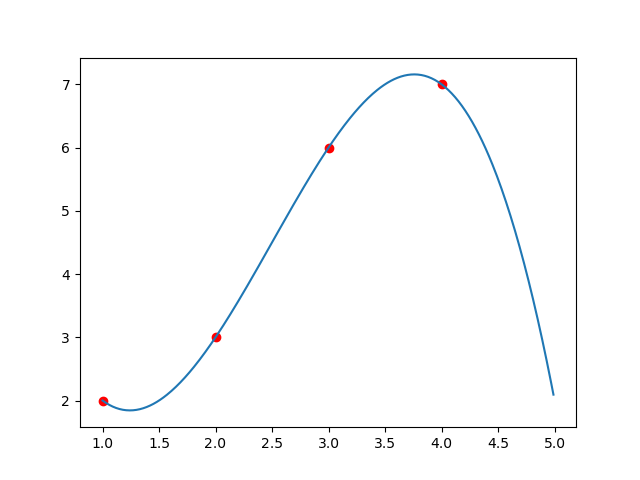
\includegraphics[width=1\linewidth]{Chapter2/graph/python/Figure2-1.png}
    \caption{Lagrange多项式插值(使用上述代码生成)}
    \label{fig:Lagrange多项式插值}
\end{figure}
\end{document}